\documentclass[english,xcolor=svgnames]{beamer}


\usepackage{mathptmx}
\usepackage[OT1]{fontenc}
% \usepackage[latin9]{inputenc}
\usepackage{amsmath}
\usepackage{amssymb}
\usepackage{amsthm}
\usepackage{mathrsfs}
\usepackage{amsfonts}
\usepackage{eurosym}
\usepackage{bm}

\usepackage{booktabs}
\usepackage{tabularx}
\usepackage{subcaption}
\usepackage[makeroom,thicklines]{cancel}

\usepackage{multirow}
\usepackage{rotating}
\usepackage{array}
\usepackage{float}



\makeatletter

 \newcommand\makebeamertitle{\frame{\maketitle}}%
 \AtBeginDocument{
   \let\origtableofcontents=\tableofcontents
 \def\tableofcontents{\@ifnextchar[{\origtableofcontents}{\gobbletableofcontents}}
   \def\gobbletableofcontents#1{\origtableofcontents}
 }
 
 \usetheme{Boadilla}
\setbeamertemplate{footline}[frame number]{}
\usefonttheme{structuresmallcapsserif}
\setbeamercolor{title}{fg=blue}
\setbeamercolor{frametitle}{fg=blue}
\setbeamercolor{caption name}{fg=blue}
\setbeamercovered{transparent}


\beamertemplatenavigationsymbolsempty

\usepackage{booktabs}
\usepackage{tabularx}
\renewcommand{\tabularxcolumn}[1]{>{\centering\arraybackslash}m{#1}}
%\newcolumntype{L}{>{\centering}X}
%\newcolumntype{H}{>{\lrbox0}c<{\endlrbox}@{}}

%\let\estinput=\input
%\newcommand{\estwide}[3]{
%          \vspace{.75ex}{
%               \begin{tabularx}
%               {\textwidth}{@{\hskip\tabcolsep\extracolsep\fill}l*{#2}{#3}}
%               \toprule
%               \estinput{#1}
%               \bottomrule
%               \addlinespace[.75ex]
%               \end{tabularx}
%               }
%          }
%
%		\newcommand{\figtext}[1]{
%		     %\vspace{-1.9ex}
%		     \captionsetup{justification=justified,font=footnotesize}
%		     \caption*{\hspace{6pt}\hangindent=1.5em #1}
%		     }
%		\newcommand{\fignote}[1]{\figtext{\emph{Note:~}~#1}}
%
\usepackage{collcell}
%\makeatother
% \newcolumntype{G}{>{\collectcell\@gobble}c<{\endcollectcell}@{}}
% \makeatother
% \def\eatcell#1\unskip{}
% \newcolumntype{E}{>{\eatcell}c@{}}
%\usepackage{tabulary}
%\usepackage{multirow}
%\usepackage{dcolumn}
%\usepackage{pdflscape}
%\usepackage{pdfpages}
% \usepackage{epsfig}
% \usepackage{epstopdf}
% \usepackage{eso-pic}
\usepackage{graphicx}
%\usepackage{arydshln}
\usepackage[compatibility=false,font={sc,rm,color=blue},justification=centering,labelformat=empty, textfont=Large, margin=2pt]{caption}
\captionsetup[figure]{belowskip=0pt}

\newcommand{\rot}[2]{\rule{1em}{0pt}%
\makebox[0cm][c]{\rotatebox{#1}{\ #2}}}

\usepackage{siunitx} %For aligning decimals
\sisetup{ detect-mode, 
          group-digits            = false ,
          input-signs             = ,
          input-symbols           = ()[]-+* ,
          input-open-uncertainty  = ,
          input-close-uncertainty = ,
          table-align-text-post   = false, 
          table-number-alignment = center
}
\selectcolormodel{cmyk}
\usepackage{color,soul}
\usepackage{colortbl}
\usepackage{tikz}
\usetikzlibrary{matrix,shapes,arrows,intersections,calc}
\usepackage{verbatim}
\setbeamercovered{invisible}
\setbeamercolor{math text displayed}{fg=blue}
\setbeamercolor{math text inlined}{fg=blue}

%\let\olditem\item
%\renewcommand{\item}{\setlength{\itemsep}{\fill}\olditem}
\AtBeginDocument{\setlength\belowdisplayskip{0pt}}


\usepackage[english]{babel}
\usepackage{booktabs}
\usepackage{tablefootnote}
\usepackage{calc,hhline,ifthen,lscape} 

%\usepackage{enumitem}
%\let\olditem\item
%\renewcommand{\item}{\setlength{\itemsep}{\fill}\olditem}

% new math commands
\newcommand{\E}{\mathbb{E}}

\newcommand{\sym}[1]{\rlap{$#1$}} %For sym in STATA tables

\setbeamertemplate{frametitle}[default][center]

% \makeglossaries
% 
% \usepackage{pgfpages}
% \pgfpagesuselayout{resize to}[a4paper, landscape, border shrink=5mm]
\usepackage[absolute,overlay]{textpos}

\usepackage{epstopdf}


%\setlength{\itemsep}{\fill}



% ===========================================================
% ===========================================================
% ===========================================================
% Improves spacing of itemize and enumerate environment

\makeatletter
\renewcommand{\itemize}[1][]{%
  \beamer@ifempty{#1}{}{\def\beamer@defaultospec{#1}}%
  \ifnum \@itemdepth >2\relax\@toodeep\else
    \advance\@itemdepth\@ne
    \beamer@computepref\@itemdepth% sets \beameritemnestingprefix
    \usebeamerfont{itemize/enumerate \beameritemnestingprefix body}%
    \usebeamercolor[fg]{itemize/enumerate \beameritemnestingprefix body}%
    \usebeamertemplate{itemize/enumerate \beameritemnestingprefix body begin}%
    \list
      {\usebeamertemplate{itemize \beameritemnestingprefix item}}
      {\def\makelabel##1{%
          {%
            \hss\llap{{%
                \usebeamerfont*{itemize \beameritemnestingprefix item}%
                \usebeamercolor[fg]{itemize \beameritemnestingprefix item}##1}}%
          }%
        }%
      }
  \fi%
  \setlength\itemsep{\fill}
    \ifnum \@itemdepth >1
        \vfill
    \fi%  
  \beamer@cramped%
  \raggedright%
  \beamer@firstlineitemizeunskip%
}

\def\enditemize{\ifhmode\unskip\fi\endlist%
  \usebeamertemplate{itemize/enumerate \beameritemnestingprefix body end}
  \ifnum \@itemdepth >1
        \vfil
  \fi%  
  }
\makeatother


\makeatletter
\def\enumerate{%
	\ifnum\@enumdepth>2\relax\@toodeep
	\else%
	\advance\@enumdepth\@ne%
	\edef\@enumctr{enum\romannumeral\the\@enumdepth}%
	\advance\@itemdepth\@ne%
	\fi%
	\beamer@computepref\@enumdepth% sets \beameritemnestingprefix
	\edef\beamer@enumtempl{enumerate \beameritemnestingprefix item}%
	\@ifnextchar[{\beamer@@enum@}{\beamer@enum@}}
\def\beamer@@enum@[{\@ifnextchar<{\beamer@enumdefault[}{\beamer@@@enum@[}}
\def\beamer@enumdefault[#1]{\def\beamer@defaultospec{#1}%
	\@ifnextchar[{\beamer@@@enum@}{\beamer@enum@}}
\def\beamer@@@enum@[#1]{% partly copied from enumerate.sty
	\@enLab{}\let\@enThe\@enQmark
	\@enloop#1\@enum@
	\ifx\@enThe\@enQmark\@warning{The counter will not be printed.%
		^^J\space\@spaces\@spaces\@spaces The label is: \the\@enLab}\fi
	\def\insertenumlabel{\the\@enLab}
	\def\beamer@enumtempl{enumerate mini template}%
	\expandafter\let\csname the\@enumctr\endcsname\@enThe
	\csname c@\@enumctr\endcsname7
	\expandafter\settowidth
	\csname leftmargin\romannumeral\@enumdepth\endcsname
	{\the\@enLab\hspace{\labelsep}}%
	\beamer@enum@}
\def\beamer@enum@{%
	\beamer@computepref\@itemdepth% sets \beameritemnestingprefix
	\usebeamerfont{itemize/enumerate \beameritemnestingprefix body}%
	\usebeamercolor[fg]{itemize/enumerate \beameritemnestingprefix body}%
	\usebeamertemplate{itemize/enumerate \beameritemnestingprefix body begin}%
	\expandafter
	\list
	{\usebeamertemplate{\beamer@enumtempl}}
	{\usecounter\@enumctr%
		\def\makelabel##1{{\hss\llap{{%
						\usebeamerfont*{enumerate \beameritemnestingprefix item}%
						\usebeamercolor[fg]{enumerate \beameritemnestingprefix item}##1}}}}}%
	\setlength\itemsep{\fill}
	\ifnum \@itemdepth >1
	\vfill
	\fi%  
	\beamer@cramped%
	\raggedright%
	\beamer@firstlineitemizeunskip%
}
\def\endenumerate{\ifhmode\unskip\fi\endlist%
	\usebeamertemplate{itemize/enumerate \beameritemnestingprefix body end}
	\ifnum \@itemdepth >1
	\vfil
	\fi%  
}
\makeatother

% ===========================================================
% ===========================================================
% ===========================================================


%\usepackage[colorlinks=true]{hyperref}

\hypersetup{colorlinks = true,linkcolor = blue, bookmarksopen=true, bookmarksopenlevel=1}

%\hypersetup{bookmarksopen=true, bookmarksopenlevel=1}

\usepackage{mathtools}

\begin{document}

\title{Monetary Policy with Heterogeneous Agents}
\vspace{1cm}
\author[shortname]{
\begin{tabular}{cc}
Juan Herre\~{n}o & Johannes Wieland \\ 
\end{tabular}\\
}



\date{UCSD, Spring \the\year}

\setbeamertemplate{footline}{}
\makebeamertitle
\setbeamertemplate{footline}[frame number]{}

\addtocounter{framenumber}{-1}

%%%%%%%%%%%%%%%%%%%%%%%%%%%%%%%%%%%%%%%%%%%%%%%%%%
\AtBeginSection[]{
\setbeamertemplate{footline}{}
  \frame<beamer>{ 

    \frametitle{Outline}   

    \tableofcontents[currentsection,hideallsubsections] 
  }
\setbeamertemplate{footline}[frame number]{}
\addtocounter{framenumber}{-1}
}

\AtBeginSubsection[]{
\setbeamertemplate{footline}{}
  \frame<beamer>{ 

    \frametitle{Outline}   

    \tableofcontents[currentsection,currentsubsection] 
  }
  \setbeamertemplate{footline}[frame number]{}
  \addtocounter{framenumber}{-1}
}



\setbeamertemplate{footline}{}
\begin{frame}
\frametitle{Outline}   
\tableofcontents[hideallsubsections] 
\end{frame}
\addtocounter{framenumber}{-1}
\setbeamertemplate{footline}[frame number]{}

\section{Introduction}
\begin{frame}{Papers}
\begin{itemize}
\item I will jump back and forth between references
\item Most of the discussion will be around Kaplan, Moll, Violante (2018)
\item I will refer to McKay, Nakamura, Steinsson (2016), and Debortoli Gali (2018) as well

\end{itemize}
\end{frame}


\begin{frame}{Motivation}
\begin{itemize}
\item Claim (proof left to the audience): Nowhere in economics the distance between theory, empirics and practice is smaller than in monetary economics
\item Mark Gertler:

\textit{Keynes famously ends the General Theory with a description of the "academic scribbler" whose ideas from "a few years back" eventually find their way into policy-making. When Marvin Goodfriend wrote "How the World Achieved Consensus on Monetary" in 2007 that time lag had largely disappeared, at least in central banking. [...] The most prominent example was the Federal Reserve chairman at the time, Ben
Bernanke. It is also now the case that the research done by staff at the Fed and other central banks is as sophisticated as any that occurs in academia.
As a result, ideas flow freely and instantly between the halls of academia and central banks. The time lag is gone.}

\end{itemize}
\end{frame}

\begin{frame}{Motivation}
\begin{itemize}
\item So what caused the explotion of acronyms ending with NK?
\begin{enumerate}
\item From Policy: Increased focus on forward guidance. The NK model predicts some really counterintuitive outcomes (forward guidance puzzle)
\item From the data: High MPCs, even for \textit{the rich hand to mouth}. NK model predicts very small MPCs out of transitory income
\item Before we go to the children (HANK, TANK, PRANK, ...), let's understand the parent (RANK)
\end{enumerate}
\end{itemize}
\end{frame}




\section{RANK}

\begin{frame}{References}
\begin{itemize}
\item From Juan's perspective: Woodford's Interest and Prices is a book you really should have
\item Gali's Monetary Policy, Inflation and Business Cycle, is a book you should probably have
\end{itemize}
\end{frame}

\begin{frame}{The three equation NK Model}
\begin{itemize}
\item The three equation model
\item Obviously everything is determined in equilibrium
\item But you can modify one block at a time
\begin{enumerate}
\item The Phillips curve. Different models get you different curves (or not)
\begin{itemize}
\item Recommendations: Gertler and Leahy (2008), Auclert, Rigato, Rognlie, Straub (2022)
\end{itemize}
\item The Taylor rule, or something more complicated. How nominal interest rates are set
\begin{itemize}
\item Large literature on discretion, commitment, optimality.
\end{itemize}
\item The inter-temporal IS curve (Euler equation): determinants of consumption growth
\end{enumerate}
\end{itemize}
\end{frame}


\begin{frame}{The Euler equation}
\begin{itemize}
\item In log-linear terms
\[\hat{c}_t = \mathbb{E}_t \hat{c}_{t+1} - \frac{1}{\gamma} (\hat{i}_t - \mathbb{E}_t \hat{\pi}_{t+1})\]
\item Notice that consumption tomorrow enters with a coefficient of 1
\item Iterate the Euler equation forward
\[\hat{c}_t = \mathbb{E}_t \hat{c}_{T} - \frac{1}{\gamma} \sum_{\tau = t}^{T} (\hat{i}_{\tau} - \mathbb{E}_t \hat{\pi}_{\tau+1})\]
\end{itemize}
\end{frame}


\begin{frame}{Forward Guidance}
\[\hat{c}_t = \mathbb{E}_t \hat{c}_{T} - \frac{1}{\gamma} \sum_{\tau = t}^{T} (\hat{i}_{\tau} - \mathbb{E}_t \hat{\pi}_{\tau+1})\]
\begin{itemize}
\item Let me assume the central bank controls the real rate
\[\hat{c}_t = \mathbb{E}_t \hat{c}_{T} - \frac{1}{\gamma} \sum_{\tau = t}^{T} \hat{r}_{\tau} \]
\item Imagine the interest rate has been $\hat{r}_t$ = 0
\item And the economy is in steady state
\item At time $t=0$ the household learns about the following policy
\[
\hat{r}_t = 
\begin{cases}
0 & \text{if $t < t^*$} \\
-\bar{r}& \text{if  $t = t^*$}\\
0 & \text{if $t > t^*$}
\end{cases}
\]
\end{itemize}
\end{frame}

\begin{frame}{The Euler equation}
\[
\hat{r}_t = 
\begin{cases}
0 & \text{if $t < t^*$} \\
-\bar{r}& \text{if  $t = t^*$}\\
0 & \text{if $t > t^*$}
\end{cases}
\]
\begin{itemize}
\item Between $t=0$ and $t=t^*$ $\hat{r}_t = 0$
\begin{itemize}
\item So $c_t = \bar{c}_1$  $\forall$ $ 0 \leq t \leq t^*]$
\end{itemize}
\item The interest rate between $t^*$ and $t^* + 1$ falls
\item the relative price of consumption fell, so you consume more in $t^*$ than in $t^*+1$
\begin{itemize}
\item So $c_{t^*+1} = \bar{c}_2 < \bar{c}_1$
\end{itemize}
\item The interest rate never changes again
\begin{itemize}
\item So $c_{t} = \bar{c}_2$ $\forall$ $t > t*$
\end{itemize}
\end{itemize}
\end{frame}

\begin{frame}{Forward Guidance}
\begin{itemize}
\item The policy we considered
\[
\hat{r}_t = 
\begin{cases}
0 & \text{if $t < t^*$} \\
-\bar{r}& \text{if  $t = t^*$}\\
0 & \text{if $t > t^*$}
\end{cases}
\]

\item Under perfect foresight
\item Creates a step-function of consumption
\[
\hat{c}_t = 
\begin{cases}
\bar{c_1} & \text{if $t \leq t^*$} \\
\bar{c_2} & \text{if $t > t^*$}
\end{cases}
\]
\item $\bar{c}_2 = 0$. Why? Monetary non-neutrality in the long-run
\item $\bar{c}_1 = \frac{1}{\gamma} \bar{r}$
\end{itemize}
\end{frame}

\begin{frame}{Forward Guidance}
\[
\hat{c}_t = 
\begin{cases}
 \frac{1}{\gamma} \bar{r} & \text{if $t \leq t^*$} \\
0 & \text{if $t > t^*$}
\end{cases}
\]
\begin{itemize}
\item So what?
\item Bizarre!
\begin{enumerate}
\item Announcing a cut tomorrow or in large $T$  has the same effect on consumption today
\item PV of CIRF of consumption is \textbf{increasing} on the horizon $t^*$
\item Forward guidance infinitely powerful on quantities
\end{enumerate}
\end{itemize}
\end{frame}

\begin{frame}{Forward Guidance}
\begin{itemize}
\item How about inflation?
\item Bizarre as well
\item Remember the iterated-forward Phillips Curve from lecture $3$
\[\pi_t =\kappa \sum_{k=0}^{\infty} \beta^k \mathbb{E}_t \hat{y}_k \]
\item In equilibrium $\hat{y} = \hat{c}$
\item Inflation response is front-loaded
\item Current inflation is increasing on the discounted sums of expected output gaps
\item Current inflation is increasing on $t^*$ keeping $\bar{r}$ fixed
\end{itemize}
\end{frame}


\begin{frame}{Mechanical intuition of the problem}
\begin{itemize}
\item The source of the problem comes from the Euler equation being extremely forward looking
\item There is no discounting in the log-linear Euler equation
\item Mechanically, if you ``discount'' the Euler equation this problem will be diminished
\item But, the source of the discounting must be convincing and appealing empirically
\end{itemize}
\end{frame}

\begin{frame}{Two possibilities (that I know of): A detour}
\begin{itemize}
\item Angeletos and Huo (2021)
\begin{itemize}
\item RA economy:
\[a_t = \varphi \xi_t  + \delta \mathbb{E}_t a_{t+1}\]
\item $a$ could be consumption in the euler equation, or $\pi$ in the PC.
\item Informational frictions (dispersed info, rational inattention)
\item The information friction outcome coincides with a representative agent economy with
\[a_t = \varphi \xi_t  + \delta \omega_f \mathbb{E}_t a_{t+1} + \omega_b a_{t-1}\]
\item for some $\omega_f < 1$ (myopia), and a $\omega_b>0$ (anchoring)
\end{itemize}
\end{itemize}
\end{frame}

\begin{frame}{Two possibilities (that I know of): Not a detour}
\begin{itemize}
\item Households out of their Euler equations
\item Borrowing constraints are a popular way of doing that
\item Speaks closely to the Keynesian cross models
\end{itemize}
\end{frame}

\begin{frame}{The intuition for HANK models}
\begin{figure}
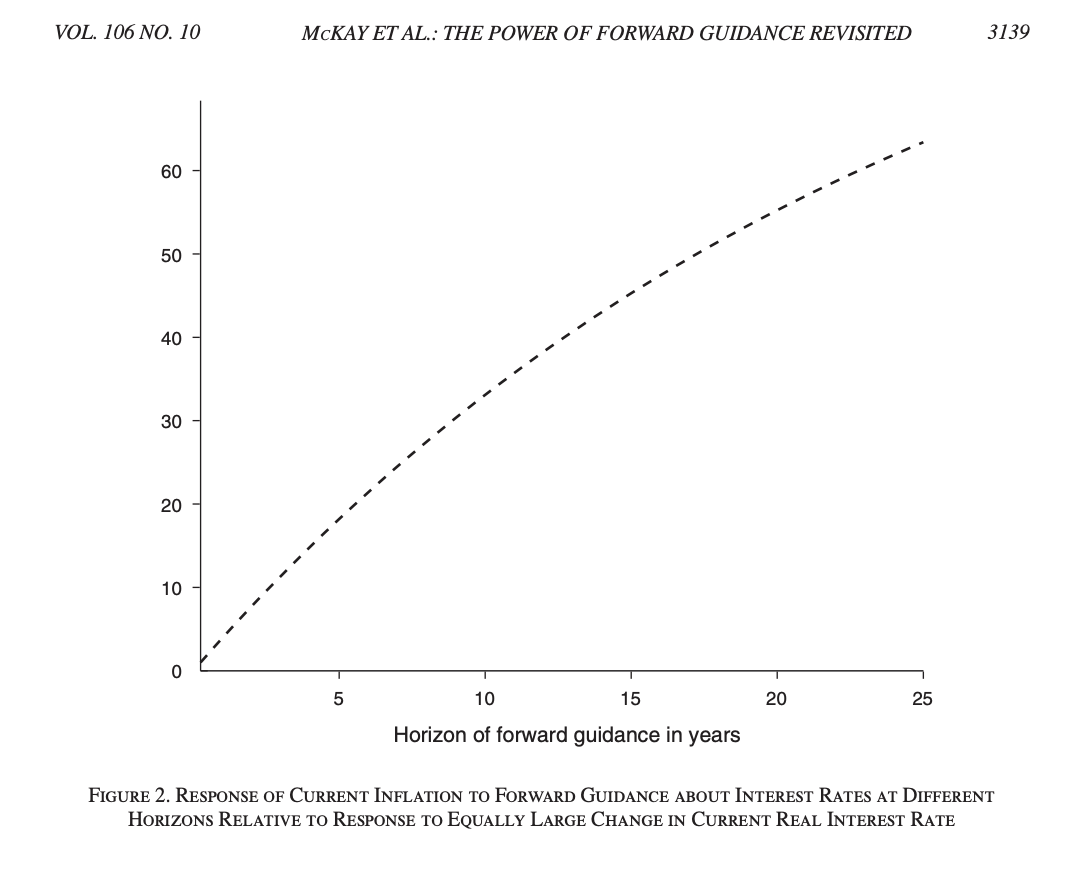
\includegraphics[scale=0.35]{figures/mns_3}\\
Source: McKay, Nakamura, Steinsson (2016)
\end{figure}
\end{frame}

\begin{frame}{The intuition for HANK models}
\begin{figure}
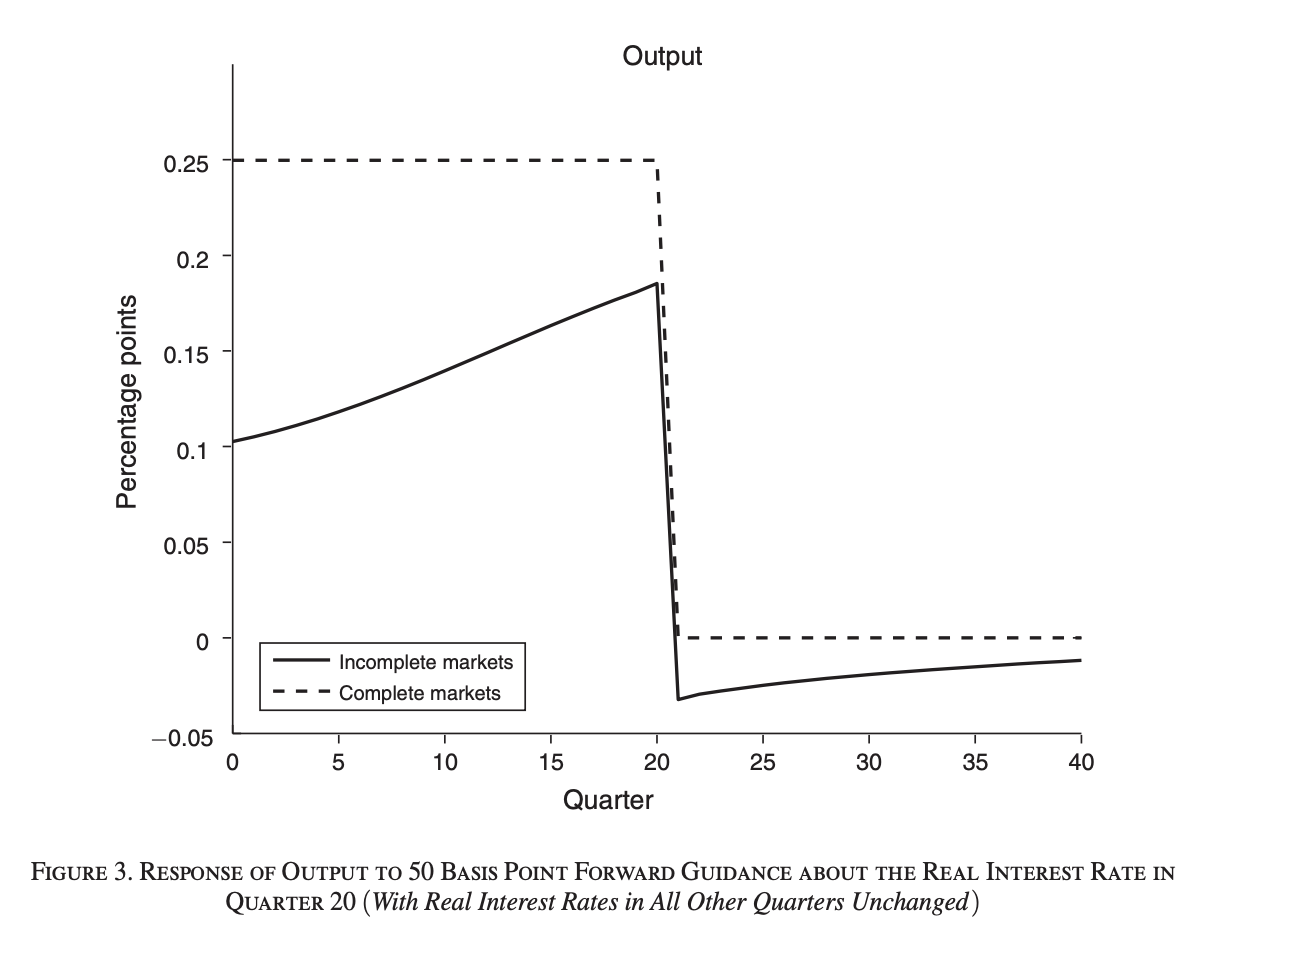
\includegraphics[scale=0.35]{figures/mns_1}\\
Source: McKay, Nakamura, Steinsson (2016)
\end{figure}
\end{frame}


\begin{frame}{The intuition for HANK models}
\begin{figure}
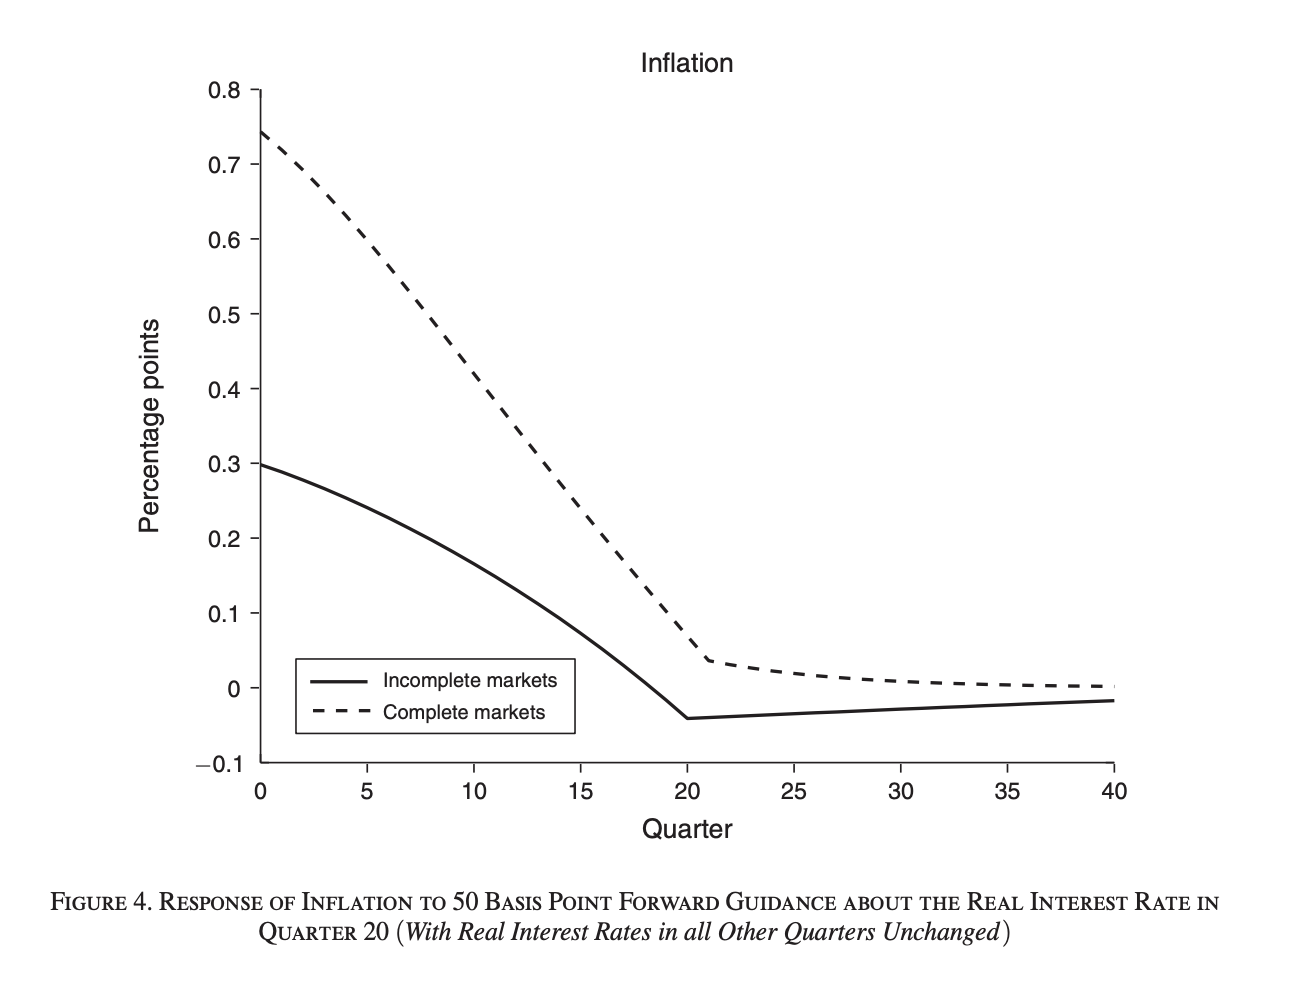
\includegraphics[scale=0.35]{figures/mns_2}\\
Source: McKay, Nakamura, Steinsson (2016)
\end{figure}
\end{frame}



\begin{frame}{The intuition for HANK models}
\begin{figure}
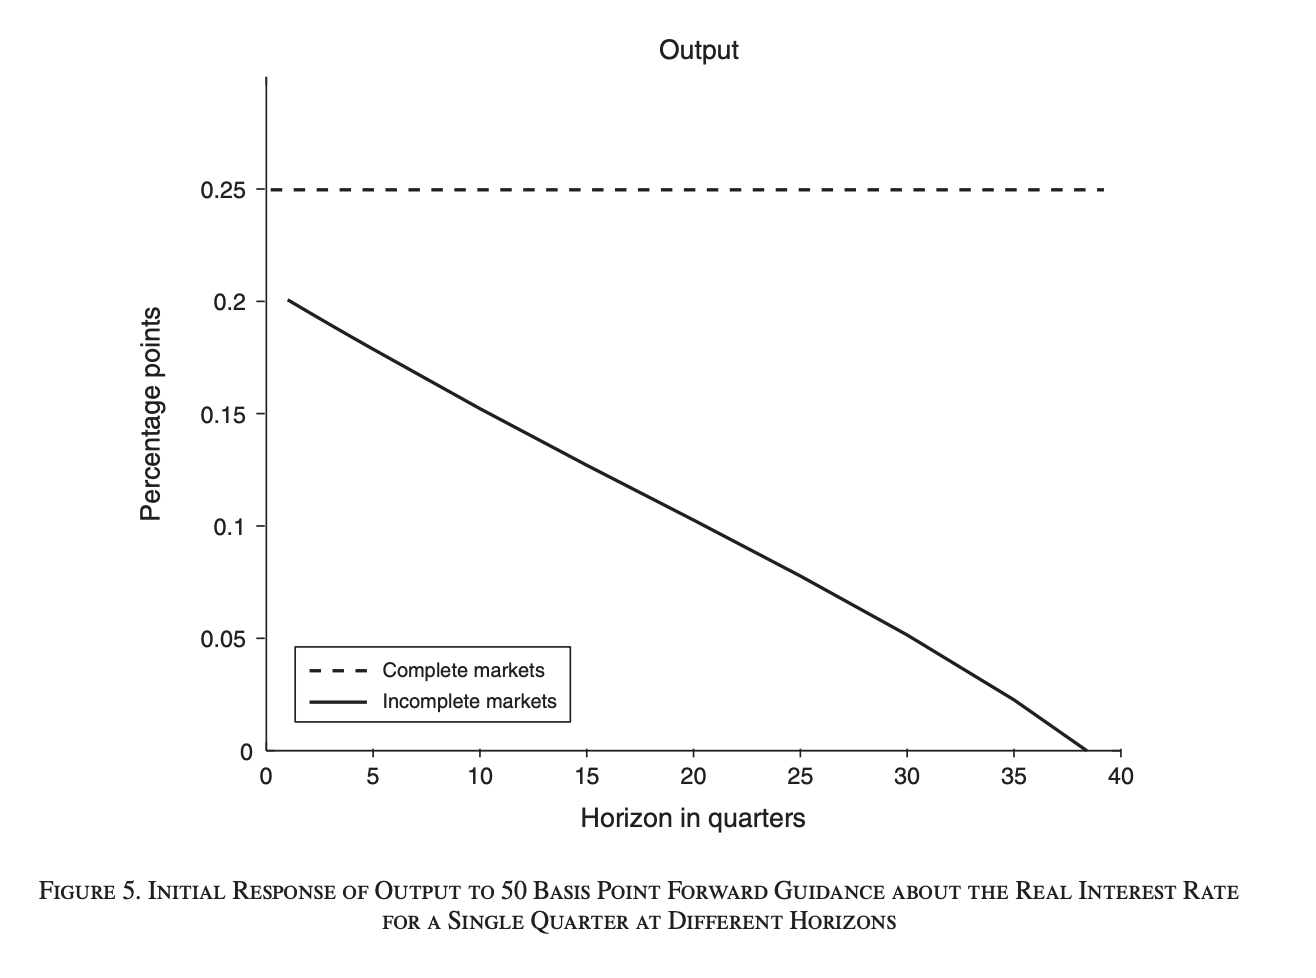
\includegraphics[scale=0.35]{figures/mns_4}\\
Source: McKay, Nakamura, Steinsson (2016)
\end{figure}
\end{frame}

\begin{frame}{The intuition for HANK models}
\begin{figure}
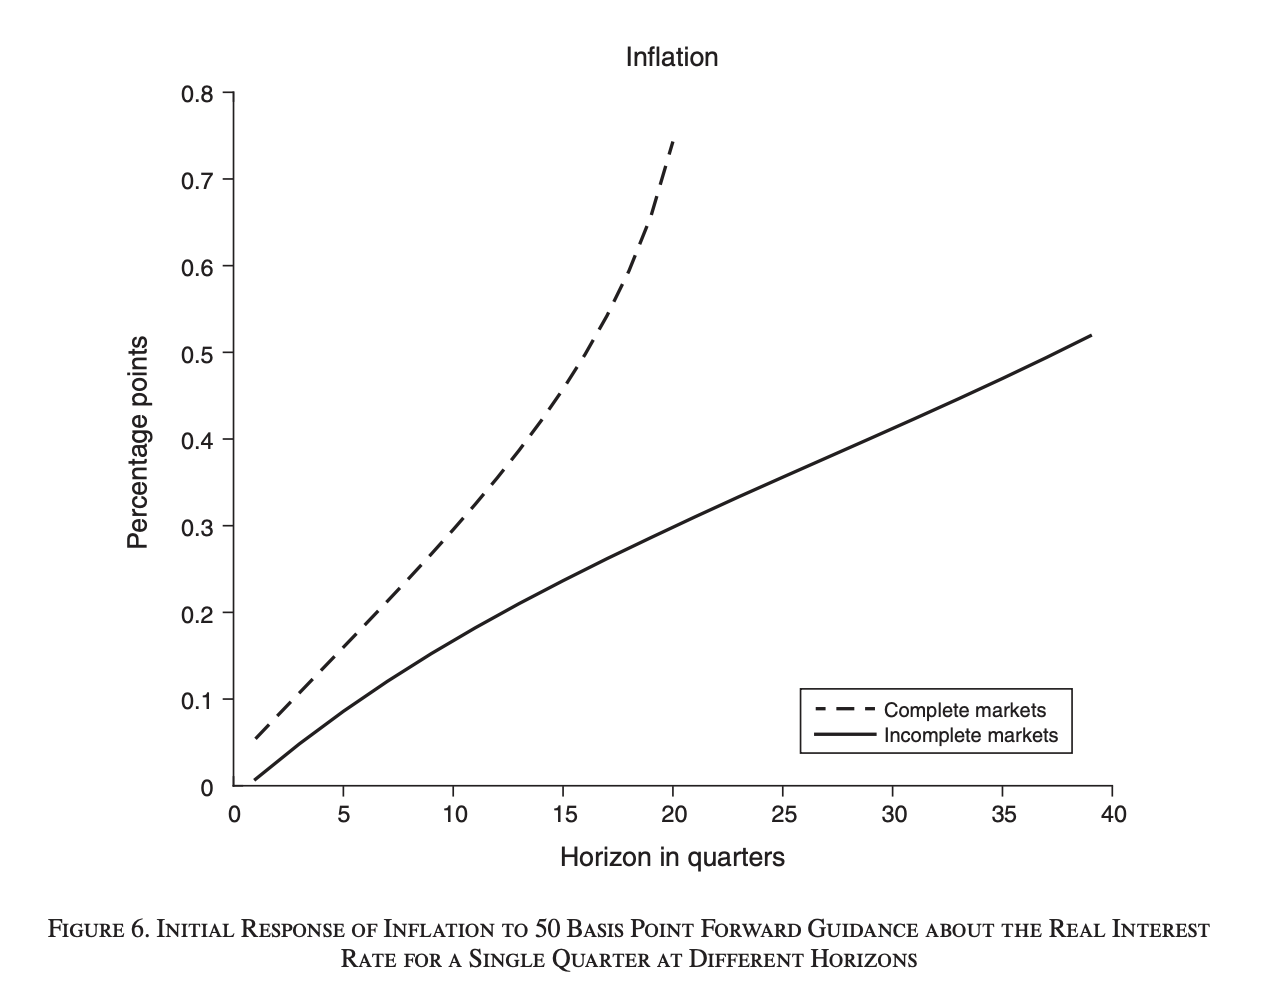
\includegraphics[scale=0.35]{figures/mns_5}\\
Source: McKay, Nakamura, Steinsson (2016)
\end{figure}
\end{frame}


\begin{frame}{Variation in MPCs}
\begin{itemize}
\item Other than the interest on the power of forward guidance, notion that MPCs out of transitory income in the RA NK model are off
\item In the textbook NK model the MPC out of transitory income is roughly zero
\item Reason: the RA in the NK model lives in the PIH world
\end{itemize}
\end{frame}

\begin{frame}{Decomposition of effects}
\begin{itemize}
\item Total differentiation of $C_0$ (on impact)
\item Similar to what we teach undergrads (tangency condition + ITBC)
\item Allowing for partial price adjustment and GE responses
\[d C_0 = \int_0^{\infty} \frac{\partial C_0}{\partial r_t} dr_t dt + \int_0^{\infty} \frac{\partial C_0}{\partial Y_t} d Y_t dt\]
\item Use a particular monetary policy rule
\[r_t  = \rho  + e^{-\eta t} (r_0 - \rho) \text{   } \forall t \geq 0 \] 
\end{itemize}
\end{frame}

\begin{frame}{Decomposition of effects}
\begin{itemize}
\item Under that policy rule (+ demand determination)
\[dC_0 = - \underbrace{\frac{1}{\gamma} \int_0^{\infty} e^{-\rho t}dr_t dt}_{\text{direct effect}} - \underbrace{\frac{\rho}{\gamma}  \int_0^{\infty} e^{-\rho t} \int_t^{\infty} d r_s ds dt}_{\text{indirect effect}} \]
\item for $\rho$ discount rate, $\eta$ persistence of the monetary policy shock
\item Can rewrite the semi-elasticity of consumption to interest rates as:
\[-\frac{d\log C_0}{dr_0} = \frac{1}{\gamma \eta} \left(\underbrace{\frac{\eta}{\eta + \rho}}_{\text{direct effect}}+ \underbrace{\frac{\rho}{\rho + \eta}}_{\text{indirect effect}}\right)\]
\item Anybody checked the proof?
\end{itemize}
\end{frame}


\section{HANK}

\begin{frame}{The HJB equation}
\begin{itemize}
\item The continuous time of the Bellman equation
\item At some point read ``Achdou, Yves, Jiequn Han, Jean-Michel Lasry, Pierre-Louis Lions, and Benjamin Moll. "Income and Wealth Distribution in Macroeconomics: A Continuous-Time Approach." The Review of Economic Studies 89, no. 1 (2022): 45-86.''
\item Perhaps in the next iteration of this lecture.
\end{itemize}
\end{frame}

\begin{frame}{The HJB equation}
\begin{multline*}
(\rho + \zeta) V(a,b,y) = \max_{c,l,d} u(c,l) + V_b(a,b,y)\dot{b} + \\ V_a(a,b,y) \dot{a} +  V_y(-\beta y) + \lambda \int_{-\infty}^{\infty}(V(a,b,x) - V(a,b,y)) \phi(x) dx
\end{multline*}
\begin{itemize}
\item $(\rho + \zeta)$ capture discounting (time and death)
\item $V_x$ is the partial derivative of the HJB with respect to $x$
\item last two terms capture the drift + jump process they assume
\[d y_{it}  = -\beta y_{it} dt + dJ_{it}\]
\item Changes in the distribution (0 in ss) are captured by a Kolmogorov Forward Equation
\end{itemize}
\end{frame}

\begin{frame}{Law of motion and financial constraints}
\begin{itemize}
\item The terms $\dot{b}$ and $\dot{a}$ in the HJB are given by
\[\dot{b}_t = (1-\tau_t) w_t z_t l_t  + r^b_t(b_t)b_t + T_t - d_t  - \chi(d_t,a_t) - c_t \]
\[\dot{a}_t =r^a_t a_t + d_t  \]
\[b_t \geq - \underline{b}\]
\[a_t \geq 0\]
\item $b$ is ``liquid''. No adjustment costs
\item $a$ is illiquid. linear and convex adjustment costs
\item Cannot short the illiquid asset
\item Borrowing limit ($\neq$ to the natural debt limit) on the liquid asset
\item is $b$ a nominal or real bond?
\end{itemize}
\end{frame}

\begin{frame}{Adjustment Costs}
\[\chi(d,a) = \chi_0 \left| d\right| + \chi_1  \left| \frac{d}{a}\right|^{\chi_2} a   \]
\begin{itemize}
\item Linear and convex costs of adjustment
\item Linear costs are obvious. Need for inaction in adjustment
\item Why do we need convex costs ($\chi_1 >0$, $\chi_2 > 1$)?
\end{itemize}
\end{frame}


\begin{frame}{Optimality conditions of HANK}
\begin{itemize}
\item Useful to characterize the FOC of the HJB equation
\item The first order condition with respect to consumption gives
\[u_c(c,l) = V_b(a,b,y)\]
\item Note there are no expectations, and no evaluations in future periods
\item One of the sources of efficiency in continuous time
\item If you can take derivatives of your guess of the value function, then back-out the policy function of consumption:
\[c = u'^{-1}(V_b(a,b,y))\]

\end{itemize}
\end{frame}

\begin{frame}{Optimality conditions of HANK}
\begin{itemize}
\item Consumption
\[u_c(c,l) = V_b(a,b,y)\]
\item Labor
\[-u_l(c,l) = V_b(a,b,y)(1-\tau)wz\]
\item Very standard
\end{itemize}
\end{frame}

\begin{frame}{Optimality conditions of HANK}
\begin{itemize}
\item Optimal deposits on illiquid asset (conditional on depositing)
\[V_a(a,b,y) = V_b(a,b,y) \chi_d(d,a)\]
\item where $\chi_d(d,a)$ is given by
\[\chi_d(d,a) = \chi_0 \frac{d}{|d|} + \chi_2 \chi_1 \frac{d}{a}\]
\item Zero convex costs when (for example) $\chi_1 = 0$
\item Pins down the deposit rate
\[\frac{V_a(a,b,y)}{V_b(a,b,y)} - \chi_0 \frac{d}{|d|} \frac{1}{\chi_1 \chi_2} = \frac{d}{a}\]
\item Without convex costs, conditional on adjustments deposits ``jump''
\item Same problem that in Q-theory models of investment
\end{itemize}
\end{frame}

\begin{frame}{Optimality conditions of HANK}
\begin{itemize}
\item When to deposit money?
\item When the value function of doing it is larger than of not doing it
\item My calculations (unchecked by anybody), deposit iff
\[ \frac{V_b(a,b,y)}{V_a(a,b,y)} \leq \frac{d}{\chi(d,a) + d}\]
\item evaluated in $d = d^*$  from the previous slide
\[\frac{V_a(a,b,y)}{V_b(a,b,y)} - \chi_0 \frac{d^*}{|d^*|} \frac{1}{\chi_1 \chi_2} = \frac{d^*}{a}\]
\end{itemize}
\end{frame}

\begin{frame}{The economics of non-convexities}
\begin{itemize}
\item I encourage you to become familiar with models of non-convexities
\item Applications:
\begin{itemize}
\item Household finance
\item Investment
\item Price-setting
\item Occupational choice
\item Technology choice
\end{itemize}
\item Happy to share my ECON 210C lecture notes applied to investment theory to those interested
\end{itemize}
\end{frame}


\begin{frame}{Firms}
\begin{itemize}
\item Competitive final good sector
\[Y_t = \left(\int_0^1 y_{jt}^{\frac{\epsilon}{\epsilon-1}}dj\right)^{\frac{\epsilon-1}{\epsilon}}\]
\item Downward sloping demand curve for each variety
\[y_{jt} = \left(\frac{p_{jt}}{P_t}\right)^{-\epsilon} Y_t\]
\item $P_t$ the ideal price index
\[P_t = \left(\int_0^1 p_{jt}^{1-\epsilon}dj\right)^{\frac{1}{1-\epsilon}}\]
\item Why do we use that price index?
\end{itemize}
\end{frame}

\begin{frame}{Price setting frictions}
\begin{itemize}
\item Rotemberg Pricing: Convex costs of changing prices. Some cool facts.
\begin{enumerate}
\item Roberts (1995) shows that the Calvo Phillips curve and the Rotemberg (1982) look the same (up to a redefinition of parameters of course)
\item Without the need to linearize around a zero-inflation steady state
\item Roberts (1995) ... for the Taylor (1979) with a change in the timing of the output gap
\item Gertler and Leahy (2008) show that a linear approx. of a Ss model looks like the Calvo model
\end{enumerate}
\end{itemize}
\end{frame}

\begin{frame}{Firm problem}
\begin{itemize}
\item Firm managers want to maximize the value of the firm
\[\int_0^{\infty} e^{- \int_0^t r^a_s ds} \left\lbrace \tilde{\Pi}_t(p_t) - \Theta\left(\frac{\dot{p_t}}{p_t}\right)\right\rbrace dt\]
\item Why do they discount profits with the rate of return of the iliquid asset?
\item No firm-specific shocks: all firms face the same marginal cost
\[m_t = \left(\frac{r^k_t}{\alpha}\right)^{\alpha} \left(\frac{w_t}{1-\alpha}\right)^{1-\alpha}\]
\item Phillips curve iterated forward
\[\pi_t  = \frac{\epsilon}{\theta} \int_t^{\infty} e^{- \int_t^s r^a_{\tau} d\tau} \frac{Y_s}{Y_t} (m_s - m^*) ds\]
\item Inflation increases following changes in expected future marginal costs
\end{itemize}
\end{frame}


\begin{frame}{Monetary Policy}
\begin{itemize}
\item Simple Taylor Rule
\[i_t = \bar{r}^b + \phi \pi_t + \varepsilon_t\]
\item $\phi > 1$ satisfying the Taylor principle
\item Fisher equation
\[r^b_t = i_t -\pi_t\]
\end{itemize}
\end{frame}

\begin{frame}{Fiscal policy}
\begin{itemize}
\item The government is the only issuer of liquid assets
\item Faces exogenous expenditures $G$
\item Imposes transfers $T$ and income taxes $\tau$
\item Satisfies an ITBC
\[\dot{B}^g_t + G_t + T_t = \tau_t \int w_t z_t l_t(a,b,y) d\mu_t + r^b_t B^g_t\]
\end{itemize}
\end{frame}

\begin{frame}{Market Clearing}
\begin{itemize}
\item Market for liquid assets clears
\[\int b d \mu_t + B^g_t = 0 \]
\item Market for illiquid assets clears
\[\int a d \mu_t = K_t + q_t \]
\item Labor market clears
\[N_t = \int z l_t(a,b,z) d \mu_t\]
\item Goods market clears
\[Y_t = C_t + I_t + G_t + \Theta_t + \chi_t + \kappa \int \max(-b,0) d\mu_t\] 
\end{itemize}
\end{frame}

\begin{frame}{Direct and indirect effects}
\begin{itemize}
\item $\Gamma$ a vector of prices $r^a,r^b,T,\tau,w$
\item Aggregate consumption integrates over households
\[C_t(\{\Gamma_t\}_{t \geq 0}) = \int c(a,b,y;\{\Gamma_t\}_{t \geq 0})d \mu_t \]
\item slight abuse of notation. The distribution $\mu$ depends on past realizations of $\Gamma$
\item Totally differentiate
\end{itemize}
\end{frame}

\begin{frame}
\begin{itemize}
\item Direct effect: due to changes in the liquid rate holding  other prices
\item Indirect effect: due to changes in other prices keeping the liquid rate
\item Direct effects are not due to temporal substitution only: there are income effects. Why?
\begin{multline*}
dC_0 = \int_0^{\infty}\frac{\partial C_0}{\partial r^b_t} dr^b_t dt + \int_0^{\infty} (\frac{\partial C_0}{\partial r^a_t} dr^a_t dt + \frac{\partial C_0}{\partial T_t} dT_t dt \\ +\frac{\partial C_0}{\partial w_t} dw_t dt + \frac{\partial C_0}{\partial \tau_t} d \tau_t dt )
\end{multline*}
\end{itemize}
\end{frame}

\begin{frame}{Small Note}
\begin{itemize}
\item I'm not aware of an easy way of computing these terms
\[\int_0^{\infty}\frac{\partial C_0}{\partial r^b_t} dr^b_t dt\]
\item This is particularly tricky in linearized RA models
\item where ``keeping constant prices'' prevents (for example) Dynare from giving you an IRF
\item You need to get these partial derivatives from the model
\[\int \frac{\partial c(a,b,y;\{r^b_t, \bar{r}^a,\bar{T},\bar{w},\bar{\tau}\}_{t \geq 0})}{\partial r^b_t}d \mu_0 dr^b_t dt \]
\item where $\mu_0$ is the partial-equilibrium model consistent cross-sectional distribution of agents
\end{itemize}
\end{frame}

\begin{frame}{Distribution of profits}
\begin{itemize}
\item What did you think?\\
\pause
\textit{Since equity is a component of illiquid assets, rather than liquid assets, the fall in profits associated with an expan- sionary monetary shock creates a downward pull on investment at a time when output is expanding. This feature is in stark contrast with the data where, quantitatively, investment is the most volatile and procyclical component of output.}
\end{itemize}
\end{frame}

\begin{frame}{Calibration}
\begin{itemize}
\item In the model, illiquid assets finance capital holdings
\item In the calibration, housing is included in illiquid asset
\item Would you improve the treatment of housing?
\end{itemize}
\end{frame}


\begin{frame}{Optimal Portfolio Choice}
\begin{itemize}
\item Liquid assets offer liquidity services
\item The volatility and persistence of earning shocks matter
\item Imagine productivity is permanent and without shocks: illiquid asset is better
\item Productivity transitory and volatile: liquid asset is better
\end{itemize}
\end{frame}

\begin{frame}{Calibration}
\begin{figure}
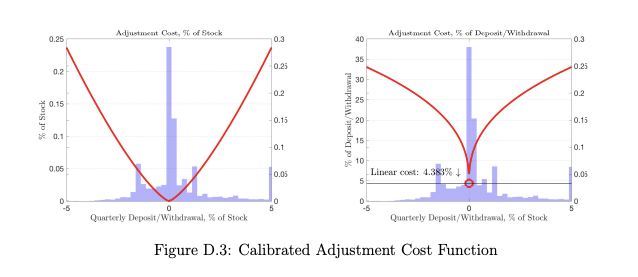
\includegraphics[scale=0.5]{figures/kmv_1}\\
Sense of how big the adjustment costs are
\end{figure}
\end{frame}

\begin{frame}{Calibration}
\begin{figure}
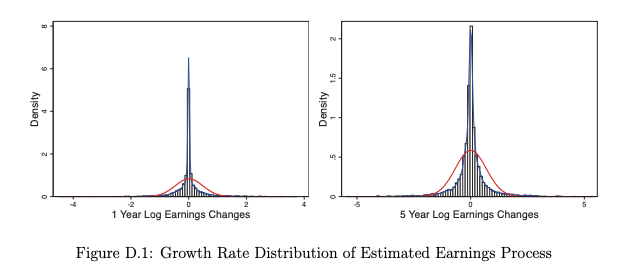
\includegraphics[scale=0.5]{figures/kmv_2}\\
The distribution of earnings shocks is leptokurtic
\end{figure}
\end{frame}


\begin{frame}{Calibration}
\begin{figure}
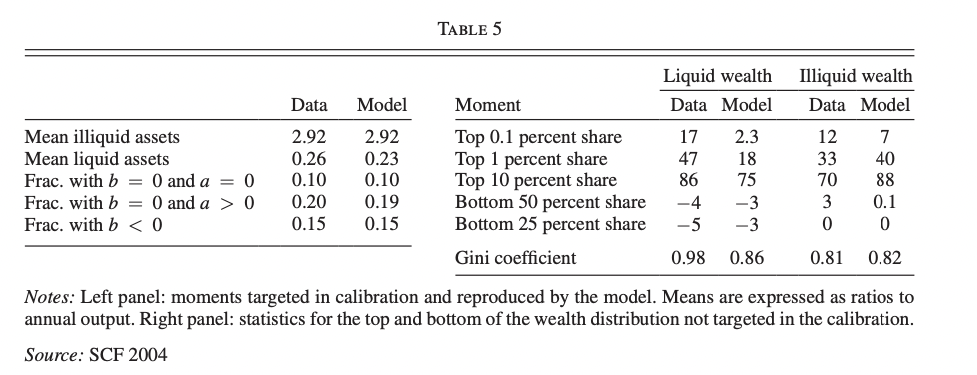
\includegraphics[scale=0.35]{figures/kmv_8}\\
Distribution of wealth holdings
\end{figure}
\end{frame}


\begin{frame}{Calibration}
\begin{figure}
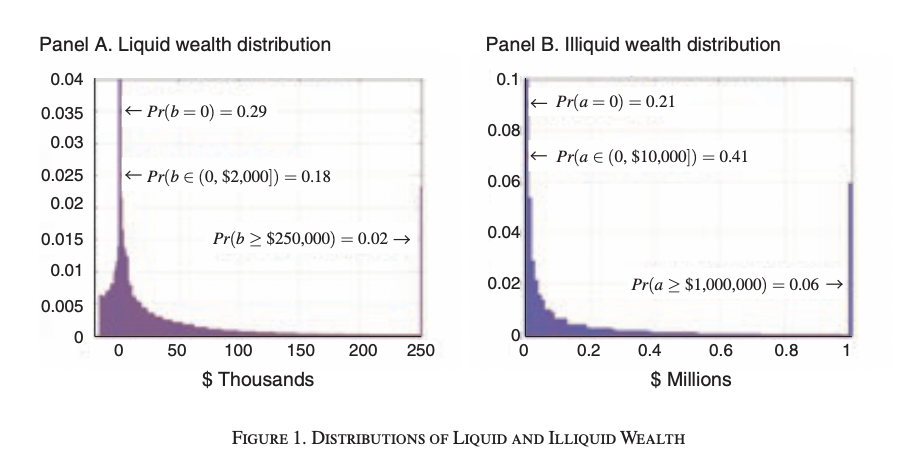
\includegraphics[scale=0.35]{figures/kmv_3}\\
Distribution of liquid and illiquid wealth
\end{figure}
\end{frame}

\begin{frame}{Calibration}
\begin{figure}
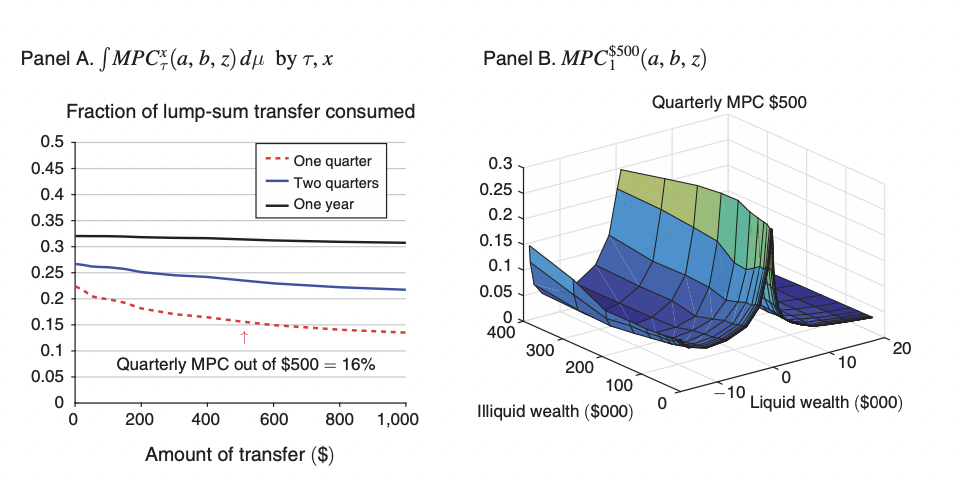
\includegraphics[scale=0.35]{figures/kmv_4}\\
Distribution of MPCs. Size dependency as in Kaplan Violante (2014)
\end{figure}
\end{frame}


\begin{frame}{Calibration}
\begin{figure}
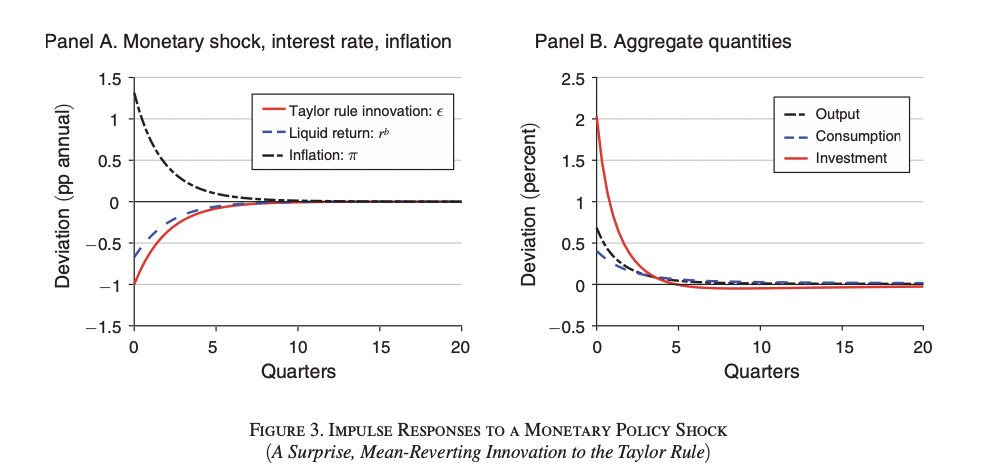
\includegraphics[scale=0.35]{figures/kmv_5}\\
Aggregate effects
\end{figure}
\end{frame}


\begin{frame}{Calibration}
\begin{figure}
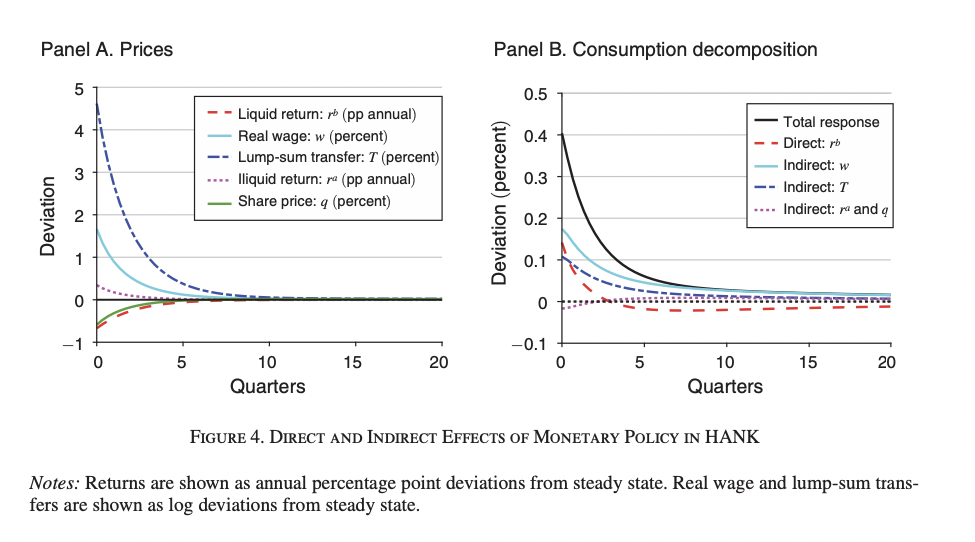
\includegraphics[scale=0.35]{figures/kmv_6}\\
Price effects and Consumption decomposition
\end{figure}
\end{frame}






\begin{frame}{Calibration}
\begin{figure}
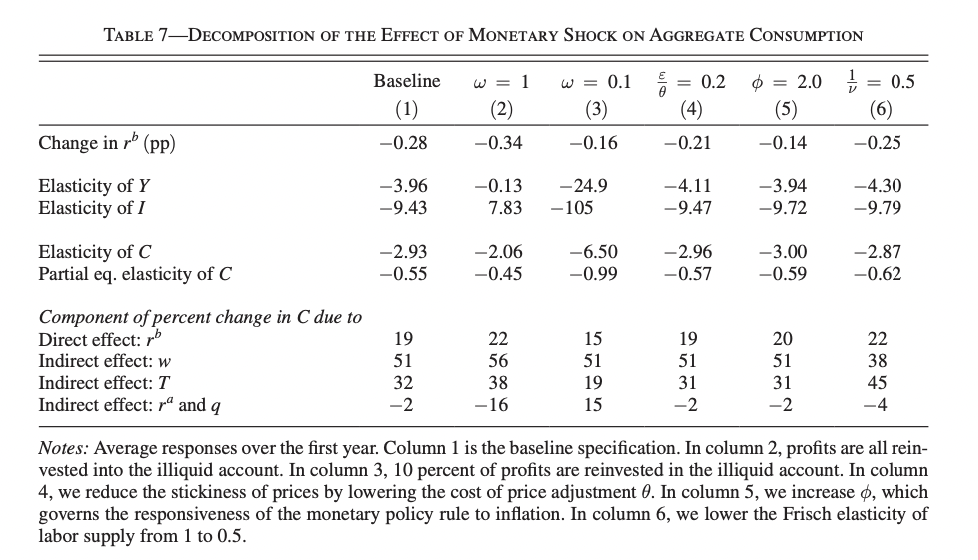
\includegraphics[scale=0.35]{figures/kmv_9}\\
Price effects and Consumption decomposition
\end{figure}
\end{frame}


\begin{frame}{Calibration}
\begin{figure}
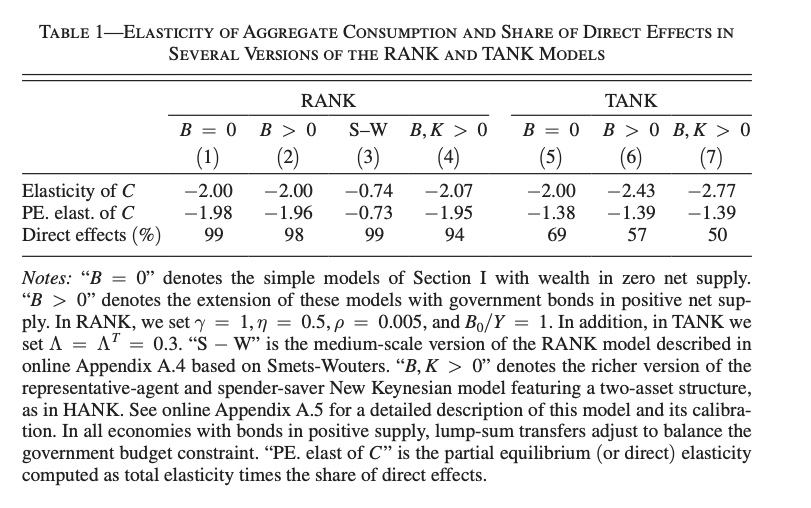
\includegraphics[scale=0.35]{figures/kmv_10}\\
Price effects and Consumption decomposition
\end{figure}
\end{frame}



\begin{frame}{Calibration}
\begin{figure}
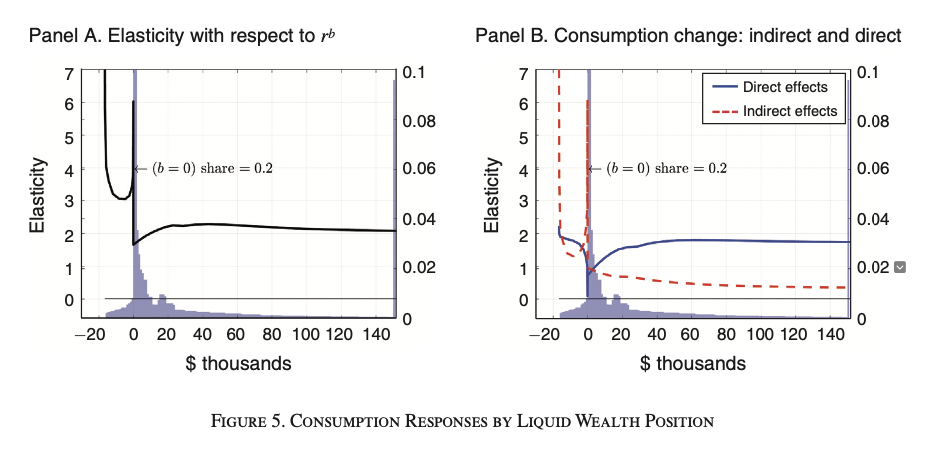
\includegraphics[scale=0.35]{figures/kmv_7}\\
Decomposition through the wealth distribution
\end{figure}
\end{frame}



\begin{frame}{Further Decomposition of the Direct Effect}
\begin{figure}
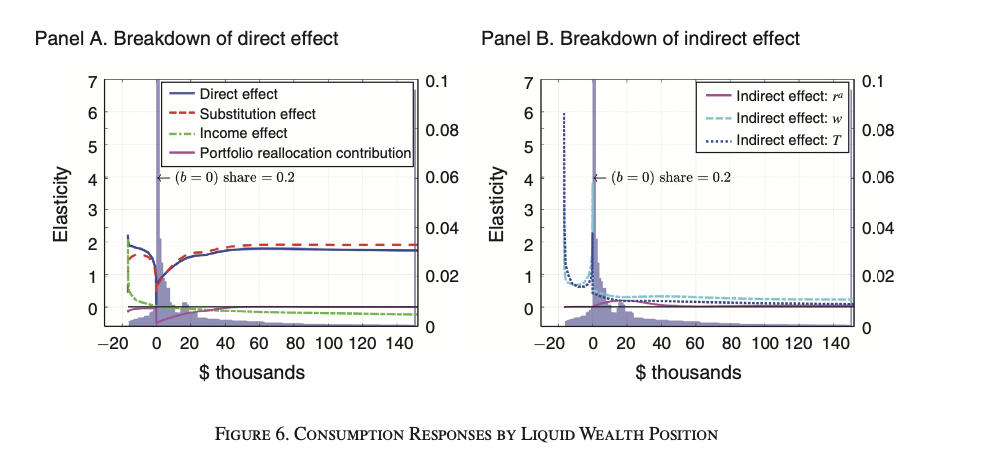
\includegraphics[scale=0.35]{figures/kmv_11}\\
Decomposition through the wealth distribution
\end{figure}
\end{frame}



\begin{frame}{Importance of Margin of adjustment}
\begin{figure}
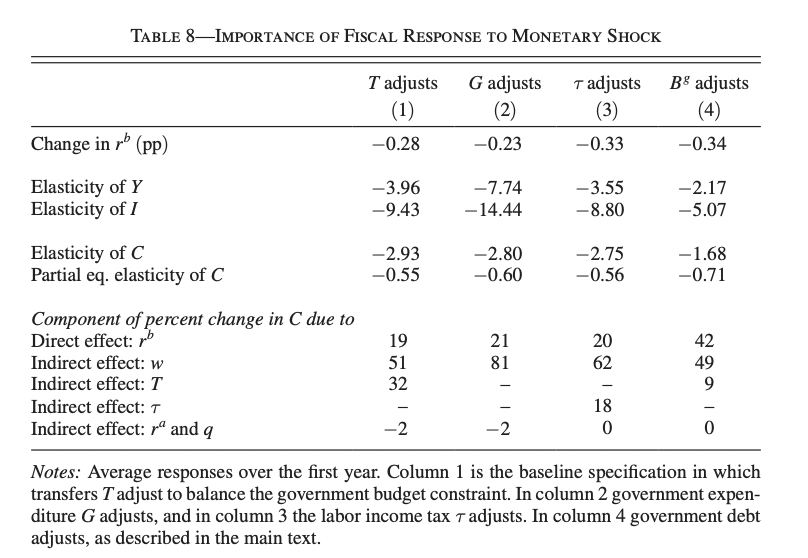
\includegraphics[scale=0.35]{figures/kmv_12}\\
Margin of fiscal adjustment
\end{figure}
\end{frame}

\begin{frame}{Why Two Assets?}
\begin{itemize}
\item The standard HA-NK model faces a tension
\item W-to-Y ratios are ``high'' (roughly 2-3)
\item MPCs are ``high''
\item Difficult to have high MPCs for wealthy people
\item Unless they cannot use their wealth to smooth consumption
\end{itemize}
\end{frame}


\begin{frame}{Persistence-Size Tradeoff}
\begin{figure}
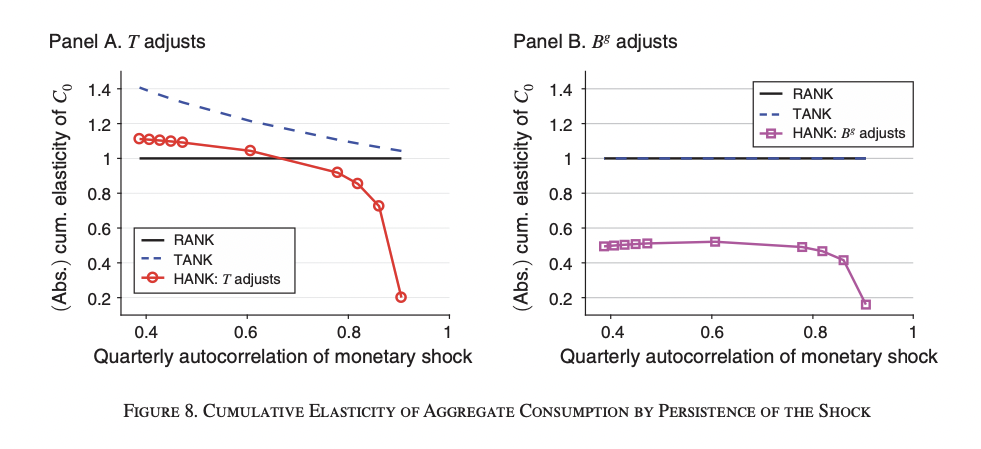
\includegraphics[scale=0.35]{figures/kmv_13}\\
Margin of fiscal adjustment
\end{figure}
\end{frame}


\section{Is TANK enough?}

\begin{frame}{Why TANK?}
\begin{itemize}
\item In HANK models borrowing constraints are not either or
\item How far are you from the constraint?
\item The probability of hitting the borrowing constraint is important
\item The problem has substantial heterogeneity
\item Simulate aggregate shocks is not trivial
\item Although Johannes will cover some neat state-of-the-art methods next week
\item Restore to simulations
\end{itemize}
\end{frame}

\begin{frame}{Is TANK enough}
\begin{itemize}
\item Metric: Is TANK close enough to HANK
\item Note that this metric is not the only potential one
\item It may be that HANK implies counterfactual behavior
\item And that TANK approximates better household behavior
\item Not the avenue that Debortoli and Gali (2016) take
\item But perhaps an interesting research possibility
\end{itemize}
\end{frame}




\begin{frame}{The simplified HANK}
\begin{itemize}
\item Here agents are hand to mouth, or unconstrained
\[\hat{c}_t = \mathbb{E}_t \hat{c}_{t+1} - \frac{1}{\gamma} \hat{r}_t - \frac{1}{\sigma}\mathbb{E}_t \Delta z_{t+1} - \mathbb{E}_t \Delta \hat{h}_{t+1}\]
\item For demand shifters $z$ and heterogeneity index $h$
\[\hat{h}_t = \hat{h}^{\gamma}_t + \hat{h}^{\theta}_t + \hat{h}^{\lambda}_t\]
\item In words: the aggregate Euler equation can differ because:
\begin{enumerate}
\item $\lambda$: The share of constrained households changes 
\item $\gamma$: A shock induces a redistribution form low to high MPC households
\item $\theta$: There is increased dispersion in consumption within a group
\end{enumerate}
\end{itemize}
\end{frame}

\begin{frame}{The TANK limit}
\begin{itemize}
\item In TANK
\[\hat{h}_t = \hat{h}^{\gamma}_t \]
\item No changes in the mass of constrained agents $h^{\lambda} = 0$
\item No dispersion within types $h^{\theta} = 0$
\item Still can have redistribution across types $h^{\gamma}$.
\end{itemize}
\end{frame}

\begin{frame}{TANK close to HANK}
\begin{figure}
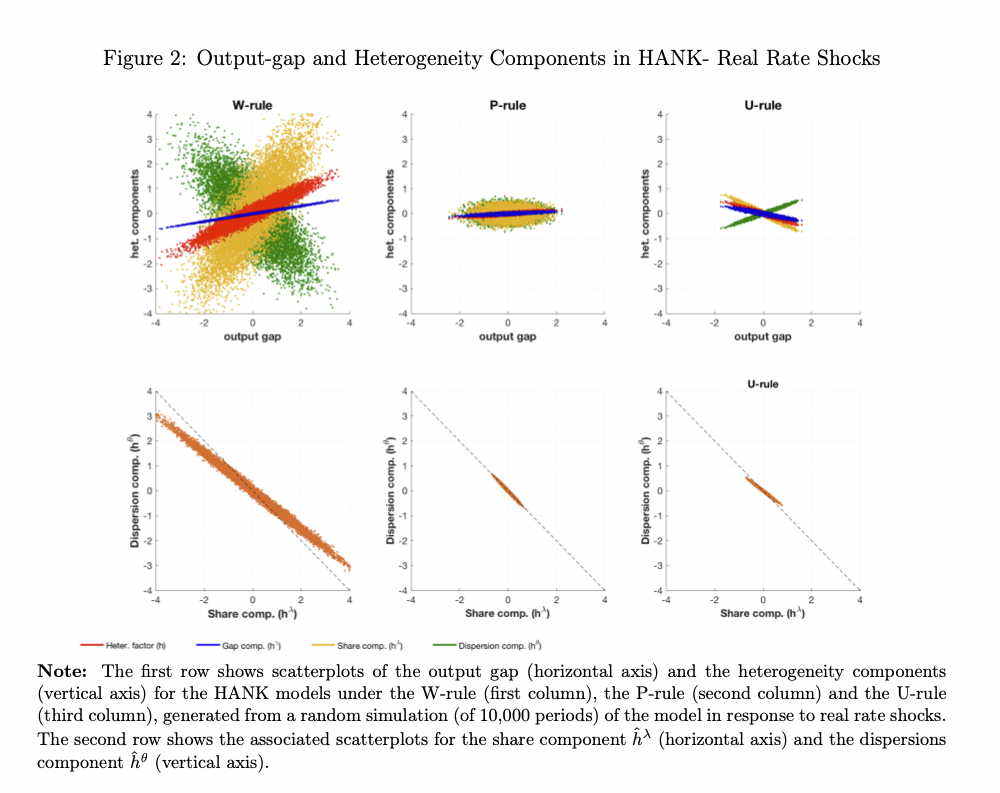
\includegraphics[scale=0.3]{figures/dg_1}
\end{figure}
\end{frame}


\begin{frame}{TANK close to HANK}
\begin{figure}
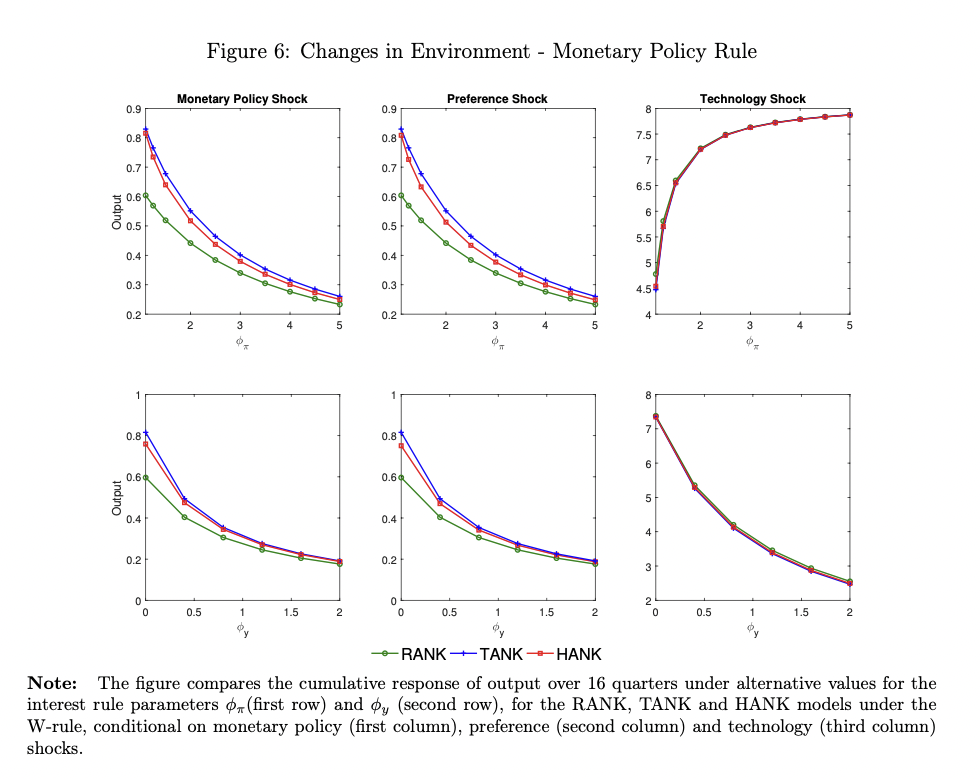
\includegraphics[scale=0.3]{figures/dg_2}
\end{figure}
\end{frame}

\begin{frame}{How I understand the paper}
\begin{itemize}
\item They are saying that the TANK model is sufficiently close to the HANK model they wrote
\item Which is different from KMV in a number of ways
\item Particularly on having households close to the borrowing constraint
\item KMV seem to claim that TANK is sufficiently far away from HANK
\item Thoughts?
\end{itemize}
\end{frame}

\section{What's on my reading list}
\begin{frame}{My HANK reading list}
	\begin{itemize}
	\item McKay and Wolf (2022): ``Optimal Policy Rules in HANK''
	\item Acharya Dogra (2020): ``Understanding HANK: Insights from a PRANK'' Econometrica, 2020, Vol 88 (May), 1113-1158\\
	\end{itemize}
\end{frame}

\end{document}

